%!Tex Root = ../Tutorat1.tex
% ./Packete.tex
% ./Design.tex
% ./Deklarationen.tex

\section{Task 1 - Memory Addresses}

\begin{frame}{Task 1 - Memory Addresses}{Task 1.1}
  \begin{solution}
    \begin{columns}
      \begin{column}{0.2\textwidth}
        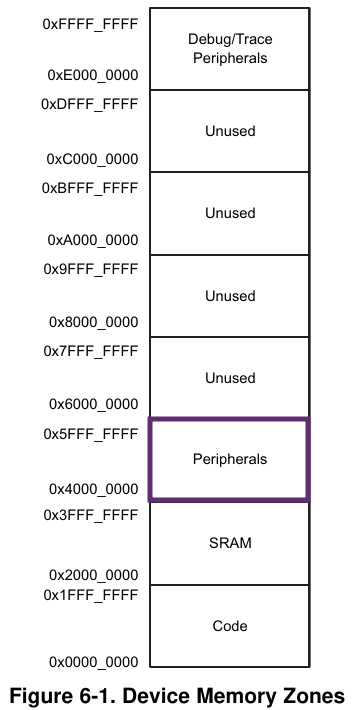
\includegraphics[height=0.5\paperheight]{./figures/peripherals.png}
      \end{column}
      \begin{column}{0.8\textwidth}
        \begin{itemize}
          \item $0x5FFF\_FFFF - 0x4000\_0000 + 1 = 0x2000\_0000$
          \item $0x2000\_0000 = 2 \cdot 16^7 = 2 \cdot {(2^4)}^7 = 2 \cdot 2^{4\cdot 7} = 2^{1+28} = 2^{29}$
        \end{itemize}
      \end{column}
    \end{columns}
  \end{solution}
\end{frame}

\begin{frame}{Task 1 - Memory Addresses}{Task 1.1}
  \begin{solution}
    \begin{columns}
      \begin{column}{0.4\textwidth}
        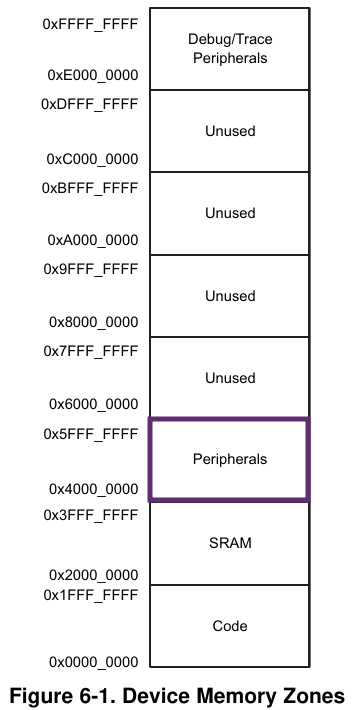
\includegraphics[height=0.5\paperheight]{./figures/peripherals.png}
        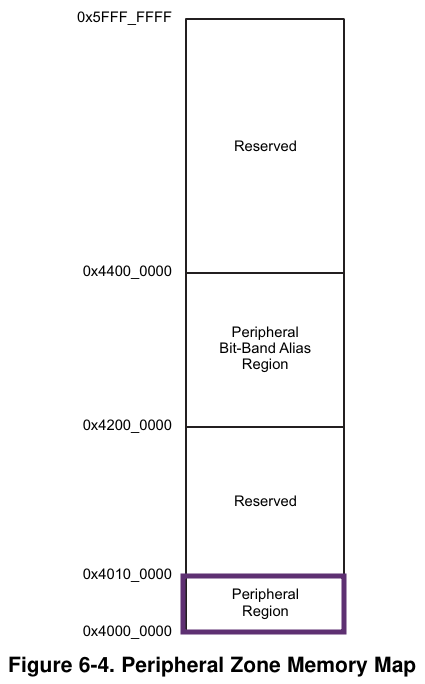
\includegraphics[height=0.5\paperheight]{./figures/peripherals_region.png}
      \end{column}
      \begin{column}{0.6\textwidth}
        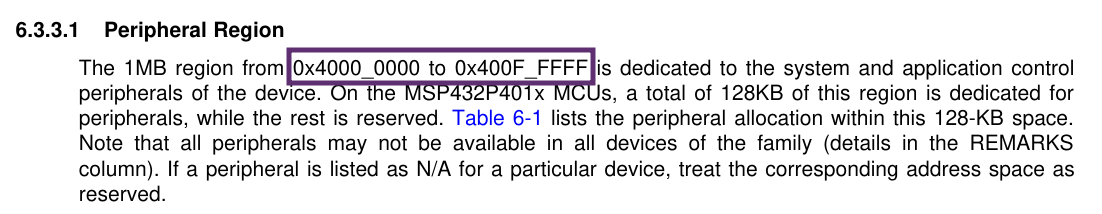
\includegraphics[width=0.5\paperwidth]{./figures/system_and_application_control_peripherals.png}
        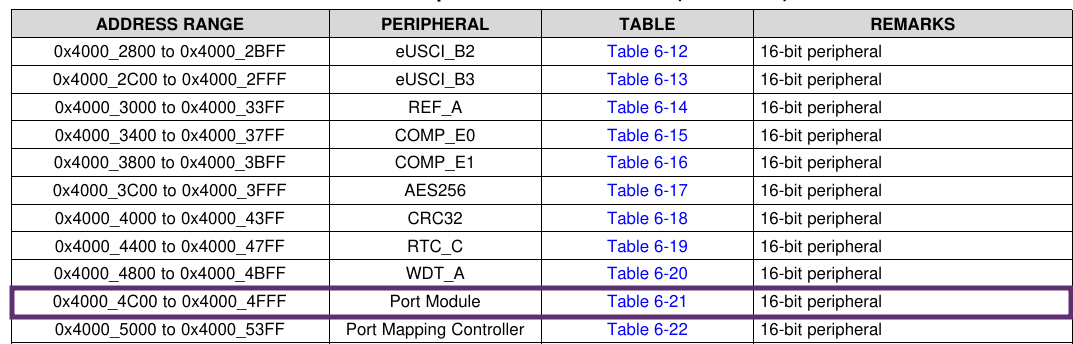
\includegraphics[width=0.5\paperwidth]{./figures/port_module.png}
      \end{column}
    \end{columns}
    \begin{itemize}
      \item $0x4000\_4FFF - 0x4000\_4C00 + 1 = 0x0400$
      \item $0x0400 = 4 \cdot 16^2 = 2^2 \cdot {(2^4)}^2 = 2^2 \cdot 2^{(4\cdot 2)} = 2^{2+8} = 2^{10}$
    \end{itemize}
  \end{solution}
\end{frame}

\begin{frame}[allowframebreaks]{Task 1 - Memory Addresses}{Task 1.1}
  \begin{solution}
    \begin{columns}
      \begin{column}{0.4\paperwidth}
        \centering
        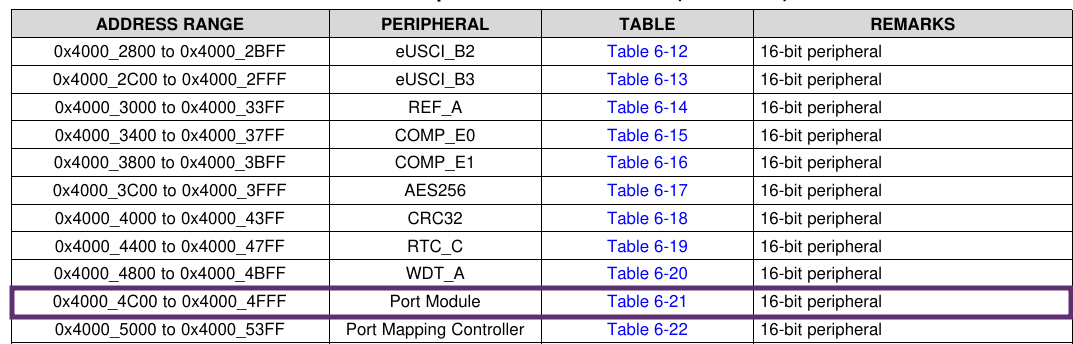
\includegraphics[width=0.3\paperwidth]{./figures/port_module.png}
        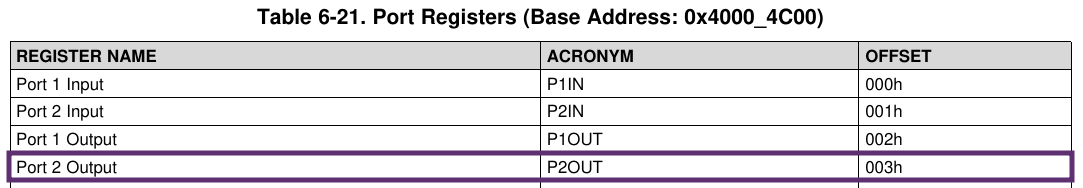
\includegraphics[width=0.3\paperwidth]{./figures/port2.png}
        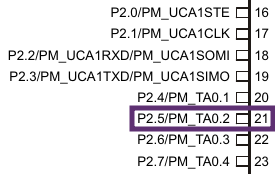
\includegraphics[height=0.2\paperheight]{./figures/2_5.png}
      \end{column}
      \begin{column}{0.6\paperwidth}
        \begin{itemize}
          \item $0x4000\_4C00 + 0x0003 = 0x4000\_4C03$
          \item 6th last significant bit $\Rightarrow$ $0b0010\_0000$
        \end{itemize}
      \end{column}
    \end{columns}
  \end{solution}
  \begin{Sidenote}
    \begin{itemize}
      \item 003h is an alternative way to wite 0x0003
    \end{itemize}
  \end{Sidenote}
\end{frame}

\begin{frame}[allowframebreaks]{Task 1 - Memory Addresses}{Task 1.1\vspace{0.25cm}}
  \begin{solution}
    \begin{columns}
      \begin{column}{0.3\paperwidth}
        \centering
        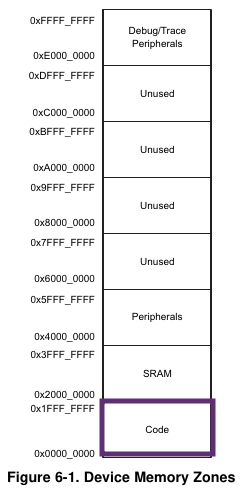
\includegraphics[height=0.4\paperheight]{./figures/code.png}
        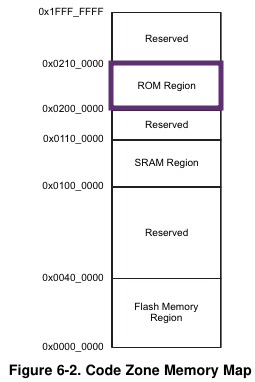
\includegraphics[height=0.4\paperheight]{./figures/rom.png}

      \end{column}
      \begin{column}{0.7\paperwidth}
        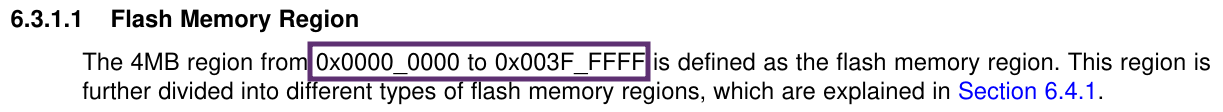
\includegraphics[height=0.095\paperheight]{./figures/rom2.png}
        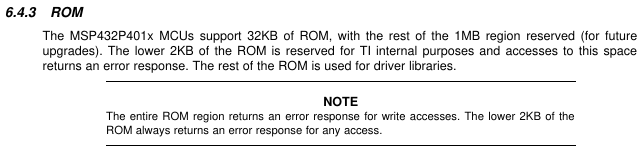
\includegraphics[height=0.25\paperheight]{./figures/rom3.png}
      \end{column}
    \end{columns}
    \begin{itemize}
      \item $0x020F\_FFFF - 0x0200\_0000 + 1 = 0x0010\_0000$.
      \item $16^5 = {(2^4)}^5 = 2^{4\cdot 5} = 2^{20} \text{addresses}$
    \end{itemize}
  \end{solution}
  \begin{solution}
    \begin{itemize}
      \item each address location corresponds to \alert{one byte} $\Rightarrow$ \alert{addressable memory space} is $2^{20} Byte$ or $1 MiB$.
      \item number of 4-byte words is a \alert{quarter} of that, which is $\frac{2^{20} Byte}{2^2} = 2^{18} words = 2^8 Kiwords= 256 Kiwords$
    \end{itemize}
  \end{solution}
  \begin{Sidenote}
    \begin{itemize}
      \item developer can not write to these addresses, only the manufacturer can (ROM = \alert{R}ead-\alert{o}nly \alert{m}emory)
      \item the MSP432P401x MCUs supports 32KB of ROM, and the rest of the 1MByte ROM region is reserved for \alert{future upgrades}
    \end{itemize}
  \end{Sidenote}
\end{frame}
